\documentclass{beamer}

\begin{document}

%%%%%%%%%%%%%%%%%%%%%%%%%%%%%%%%%%%%%%%%%%%%%%%%%%%

\begin{frame}
\frametitle{Changing boundaries of geographic units}
Applied work often uses data with a spatial component
\begin{itemize}
    \item counties
    \item commuting zones
    \item congressional districts
    \item ...
\end{itemize}
\bigskip

Either you want to
\begin{itemize}
    \item have consistent spatial units over time (e.g.\ changing county boundaries across Census years)
    \item combine data from different spatial units (e.g.\ construct variables for congressional districts using county-level information)
\end{itemize}

\end{frame}

%%%%%%%%%%%%%%%%%%%%%%%%%%%%%%%%%%%%%%%%%%%%%%%%%%%

\begin{frame}
\frametitle{Area-based harmonization methods}
\begin{itemize}
    \item Suppose you want to get county information (e.g.\ total income) for congressional districts (CD); use stock variables, not shares, you can build shares and percentages \textbf{after} the boundary harmonization
    \pause
    \item Hornbeck (2010) pioneered the following procedure
    \begin{enumerate}
        \item Using ArcGIS (or other mapping software), intersect the CD boundaries with all counties or parts of counties which fall into a given CD
        \item Take total income in each county and sum it within the CD
        \begin{itemize}
            \item counties solely lying in that CD receive a weight of 1
            \item counties that partially lie in that CD receive a weight of $\frac{a}{A}$, where $a$ is the area of the county that lies in the CD and $A$ is the total area of the county
        \end{itemize}
    \end{enumerate}
    \pause
    \item The last step assumes that total income is uniformly distributed across the county area
    \begin{itemize}
        \item this will not hold in the presence of \textbf{urbanization/agglomeration} economies to the extent that origin and reference unit boundaries intersect
    \end{itemize}
\end{itemize}

\end{frame}

%%%%%%%%%%%%%%%%%%%%%%%%%%%%%%%%%%%%%%%%%%%%%%%%%%%

\begin{frame}
\begin{figure}
    \centering
    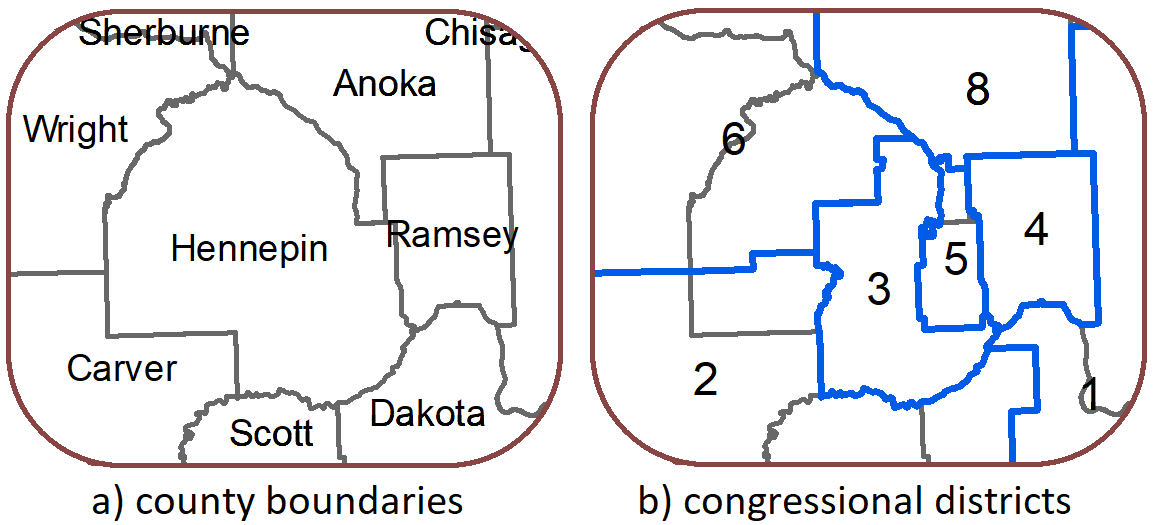
\includegraphics[width=0.75\textwidth]{figures/counties_CDs.png}
\end{figure}
\begin{itemize}
    \item CD3: $\frac{\text{Area}_{\text{CD3}}}{\text{Area}_{\text{Hennepin}}}\times (\text{total income}_{\text{Hennepin}})$ since CD3 is entirely in Hennepin county \pause
    \item CD5: $\frac{\text{Area}_{\text{CD5 in Hennepin}}}{\text{Area}_{\text{Hennepin}}}\times (\text{total income}_{\text{Hennepin}}) + \frac{\text{Area}_{\text{CD5 in Anoka}}}{\text{Area}_{\text{Anoka}}}\times (\text{total income}_{\text{Anoka}})$, since CD5 covers parts of both Hennepin and Anoka \pause
    \item Total income in CD 2/4/6/8 are the weighted sums of total income from counties and county parts belonging to these CDs.
\end{itemize}

\end{frame}

%%%%%%%%%%%%%%%%%%%%%%%%%%%%%%%%%%%%%%%%%%%%%%%%%%%

\begin{frame}
\begin{figure}
    \centering
    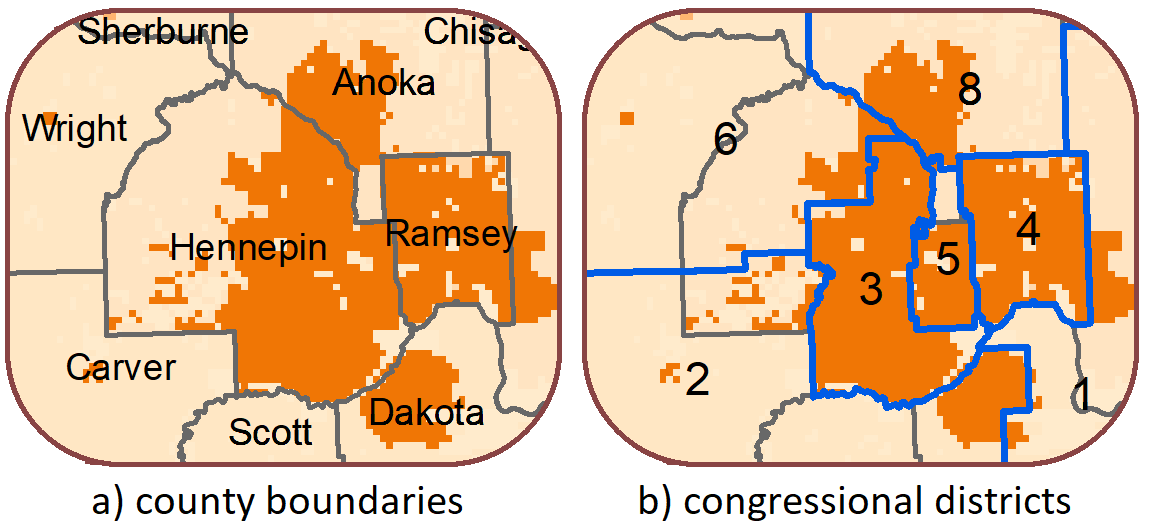
\includegraphics[width=0.75\textwidth]{figures/counties_CDs_pop.png}
\end{figure}
\begin{itemize}
    \item But new population data by Fang and Jawitz (2018) shows that population is not uniformly distributed within counties
    \begin{itemize}
        \item they develop different spatial models for 1$\times$1km grid cell population distributions from 1790 to 2010
        \item yellow and orange are approximately above/below mid-range population (for simplicity)
    \end{itemize}
\end{itemize}

\end{frame}

%%%%%%%%%%%%%%%%%%%%%%%%%%%%%%%%%%%%%%%%%%%%%%%%%%%

\begin{frame}
\frametitle{New population-based crosswalks}
\begin{itemize}
    \item Using this new population data, Ferrara, Testa, and Zhou (2021) provide a complementary approach to Hornbeck (2010) with new crosswalks for
    \begin{itemize}
        \item counties-to-counties over time (Census decades)
        \item Counties-to-congressional districts
    \end{itemize}
    \item from 1790 to 2020 using population-based weights instead of area-   
   based weights. The crosswalks can be downloaded at \\ \color{blue}\url{https://doi.org/10.3886/E150101}\color{black}
\end{itemize}
\bigskip
\begin{itemize}
    \item How much does adjusting for population distribution matter?
\end{itemize}

\end{frame}

%%%%%%%%%%%%%%%%%%%%%%%%%%%%%%%%%%%%%%%%%%%%%%%%%%%

\begin{frame}
\frametitle{Comparison with actual CD-level data}

\begin{itemize}
    \item Ferrara, Testa and Zhou (2021) take official Census data for CDs which exist for 1960, 1970, 1980 and 1980
    \item They generate CD-level variables from county-level data using
    \begin{itemize}
        \item area-based weights (model M1)
        \item population-based weights (models M2-4)
        \item (slight differences between M2-4 in how the sub-county population distribution is generated; in practice it makes little difference)
    \end{itemize}
    \item And then they compare how closely the different crosswalks can replicate the official data (next slide)
    \begin{itemize}
        \item relative to M1, M2-4 have a \textbf{20\% higher correlation} with the official CD data
    \end{itemize}
\end{itemize}

\end{frame}

%%%%%%%%%%%%%%%%%%%%%%%%%%%%%%%%%%%%%%%%%%%%%%%%%%%

\begin{frame}
\begin{figure}
    \centering
    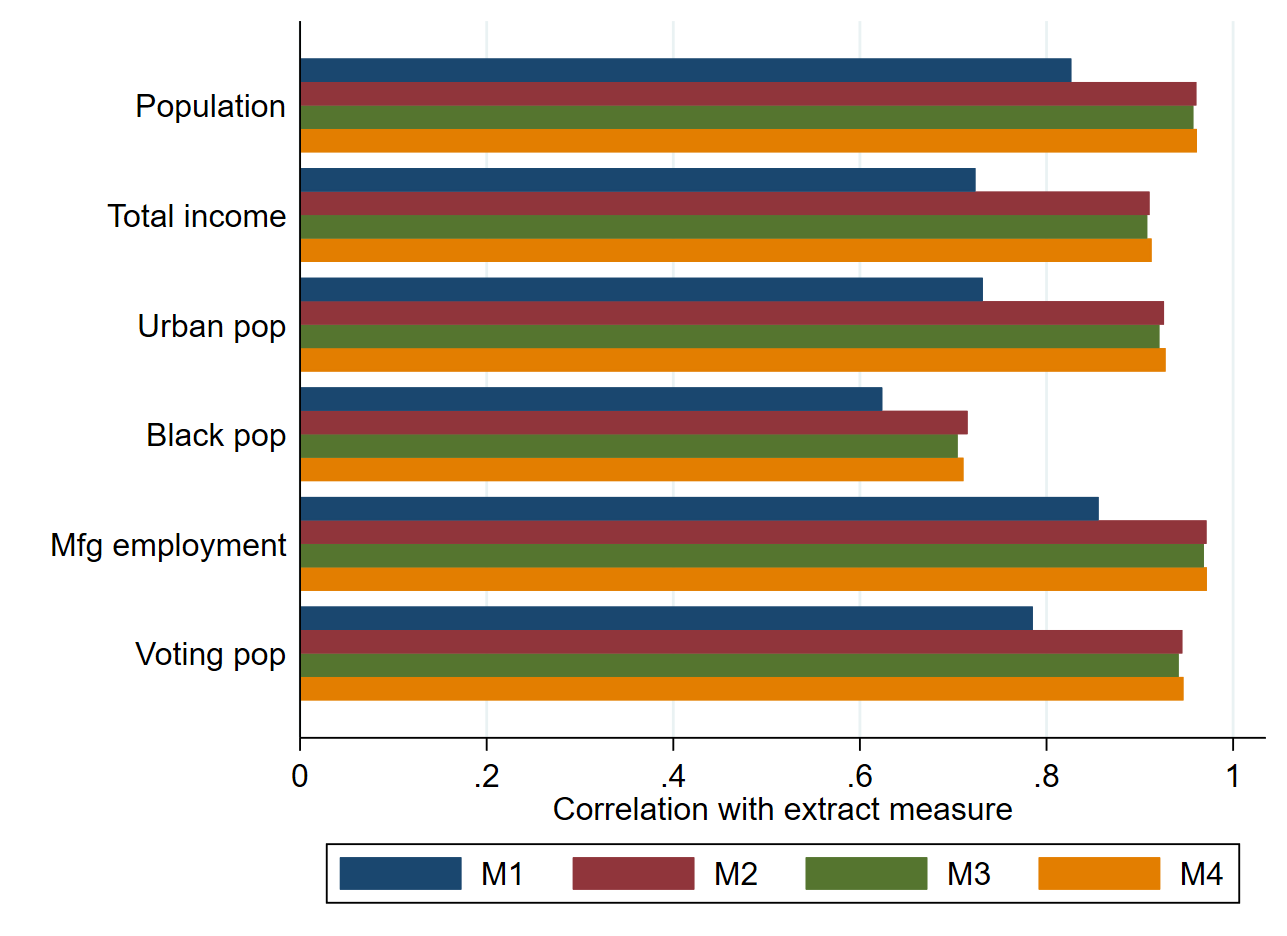
\includegraphics[width=\textwidth]{figures/LMB_model_correlations.png}
\end{figure}

\end{frame}

%%%%%%%%%%%%%%%%%%%%%%%%%%%%%%%%%%%%%%%%%%%%%%%%%%%

\begin{frame}
\frametitle{Assumptions and caveats}

\begin{itemize}
    \item Of course, there are still some assumptions and caveats
    \begin{itemize}
        \item Fang and Jawitz (2018) still rely on \textbf{uniformity within defined urban and rural areas} (though this is relaxed further in M4)
        \item earlier Census years increasingly rely on mathematical assumptions about urban extents over official Census data from the year 2000; this may not be unreasonable given that city population growth tends to follow certain power distributions (see Chen, 2015), but it is important to pick a reference year that pre-dates any ``treatment''
        \item population-based approaches \textbf{work well for stock variables that are correlated with population}, like income, number of workers, etc. If a variable is inversely correlated with population, say air quality, then population-based weights can be worse than area-based ones
        \begin{itemize}
            \item Solution: turn variable into something that correlates positively with population (e.g.\ use air pollution instead of air quality)
        \end{itemize}
    \end{itemize}
\end{itemize}

\end{frame}

%%%%%%%%%%%%%%%%%%%%%%%%%%%%%%%%%%%%%%%%%%%%%%%%%%%

\begin{frame}
\frametitle{How to apply the crosswalks}
\begin{itemize}
    \item Suppose you want to harmonize county level data on the stock of Mexican-born population in 1960 to the 88th CDs
    \begin{enumerate}
        \item Get the county-level data for 1960 for the total number of persons born in Mexico. It is critical to harmonize only county-level stock variables for weights to be appropriate
        \item Given some set of county identifiers (e.g.\ FIPS or NHGIS codes), merge the 1960 county file with the 1960 to 88th Congress crosswalk file
        \item Multiply the number of persons born in Mexico with the provided weights
        \item Finally, collapse (i.e.\ sum) the weighted counts for each variable by CD identifiers. Round or mark as missing any cell as needed. The unit of observation is now the CD level
    \end{enumerate}
\end{itemize}

\end{frame}

%%%%%%%%%%%%%%%%%%%%%%%%%%%%%%%%%%%%%%%%%%%%%%%%%%%

\begin{frame}
\frametitle{References}

\begin{itemize}
    \item Chen, Y.\ ``The distance-decay function of geographical gravity model: Power law or exponential law?'', Chaos, Solutions \& Fractals, Vol.\ 77, pp. 174-189.
    \item Fang, Y.\ and Jawitz, J.W.\ (2018) ``High-resolution reconstruction of the United States human population distribution, 1790 to 2010'', Scientific Data, Vol.\ 5, \url{https://doi.org/10.1038/sdata.2018.67}.
    \item Ferrara, A., Testa, P., and Zhou, L.\ (2021) ``New Area- and Population-based Geographic Crosswalks for U.S. Counties and Congressional Districts, 1790-2020'', CAGE Working Paper No. 588.
    \item Hornbeck, R.\ (2010) ``Barbed Wire: Property Rights and Agricultural Development'', Quarterly Journal of Economics, Vol.\ 125(2), pp. 767-810.
\end{itemize}

\end{frame}

%%%%%%%%%%%%%%%%%%%%%%%%%%%%%%%%%%%%%%%%%%%%%%%%%%%


\end{document}